Là phương pháp mô hình hóa biến thiên 2D theo thời gian để phân tích chuỗi thời gian tổng quát. Hành động tách các khoảng thời gian khác nhau khỏi chuỗi thời gian có thể làm giảm đáng kể độ phức tạp để xử lý các mô hình.

\begin{figure}[htbp]
\centerline{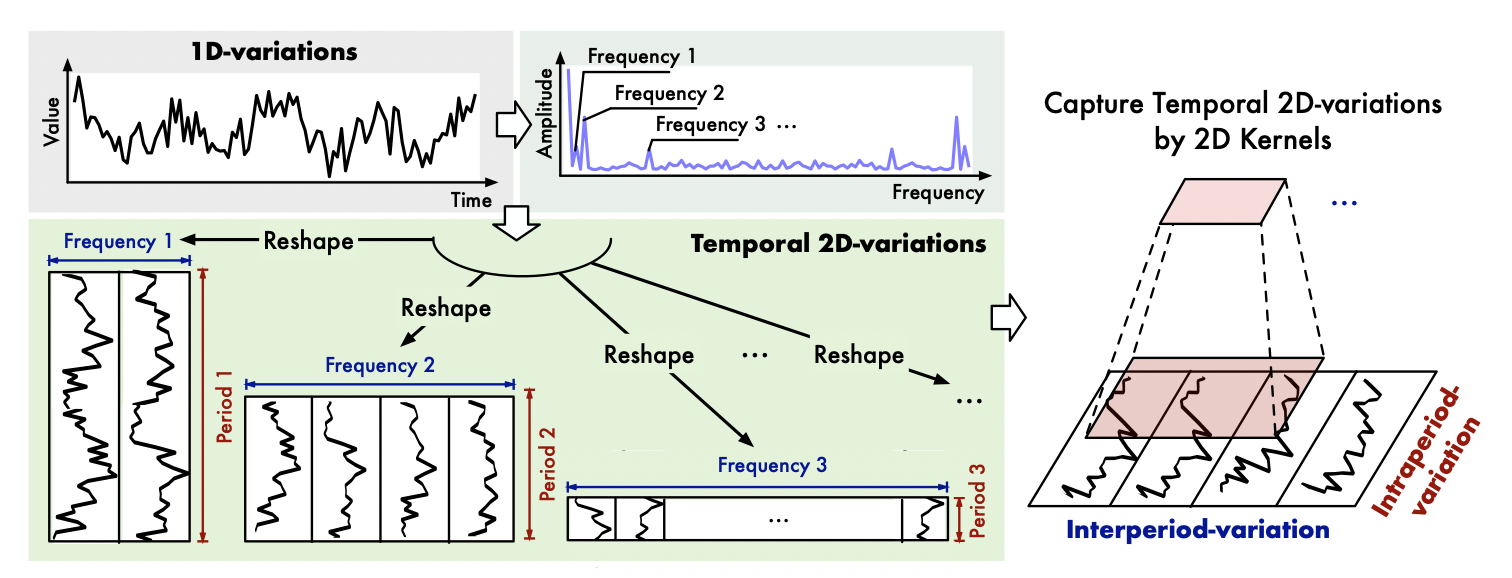
\includegraphics[width=0.4\textwidth]{img/2Dstructure.png}}
\caption{Minh họa cấu trúc 2D trong chuỗi thời gian.}
\label{fig}
\end{figure}

Chuỗi thời gian 1D được chuyển đổi thành nhiều tensor 2D. Mỗi tensor đại diện cho một chu kỳ cụ thể được xác định thông qua quá trình FFT. Việc biến đổi này được điều chỉnh bởi các phương trình sau:
\[
X_f=FFT(X)
\]
\[
A_f=\frac{1}{d}\sum\limits_{i=1}^d\mid X_f[i]\mid
\]
\[
P_k=\frac{T}{k}
\]
\[
X_{2D}^{(k)}= reshape(X, P_k)
\]
Trong đó:\\
    \indent\textbullet\ \(X\): chuỗi thời gian ban đầu.\\
    \indent\textbullet\ \(X_f\): đại diện cho FFT của nó.\\
    \indent\textbullet\ \(A_f\): phổ biên độ.\\
    \indent\textbullet\ \(P_k\): độ dài chu kỳ cho tần số k.\\
    \indent\textbullet\ \(X_{2D}^{(k)}\):  tensor 2D được định hình lại cho chu kỳ.\\

TimesNet sử dụng một kiến trúc mô-đun với nhiều TimesBlock, mỗi khối được thiết kế để xử lý các tensor 2D và nắm bắt các biến thiên thời gian. Một TimesBlock được định hình như sau:
\[
H_{l+1}=F(H_l)+H_l
\]
Trong đó:\\
    \indent\textbullet\ \(H_l\): đầu vào cho TimesBlock thứ l.\\
    \indent\textbullet\ \(F\): biểu thị chuỗi các biến đổi được áp dụng trong khối.
    
\begin{figure}[htbp]
\centerline{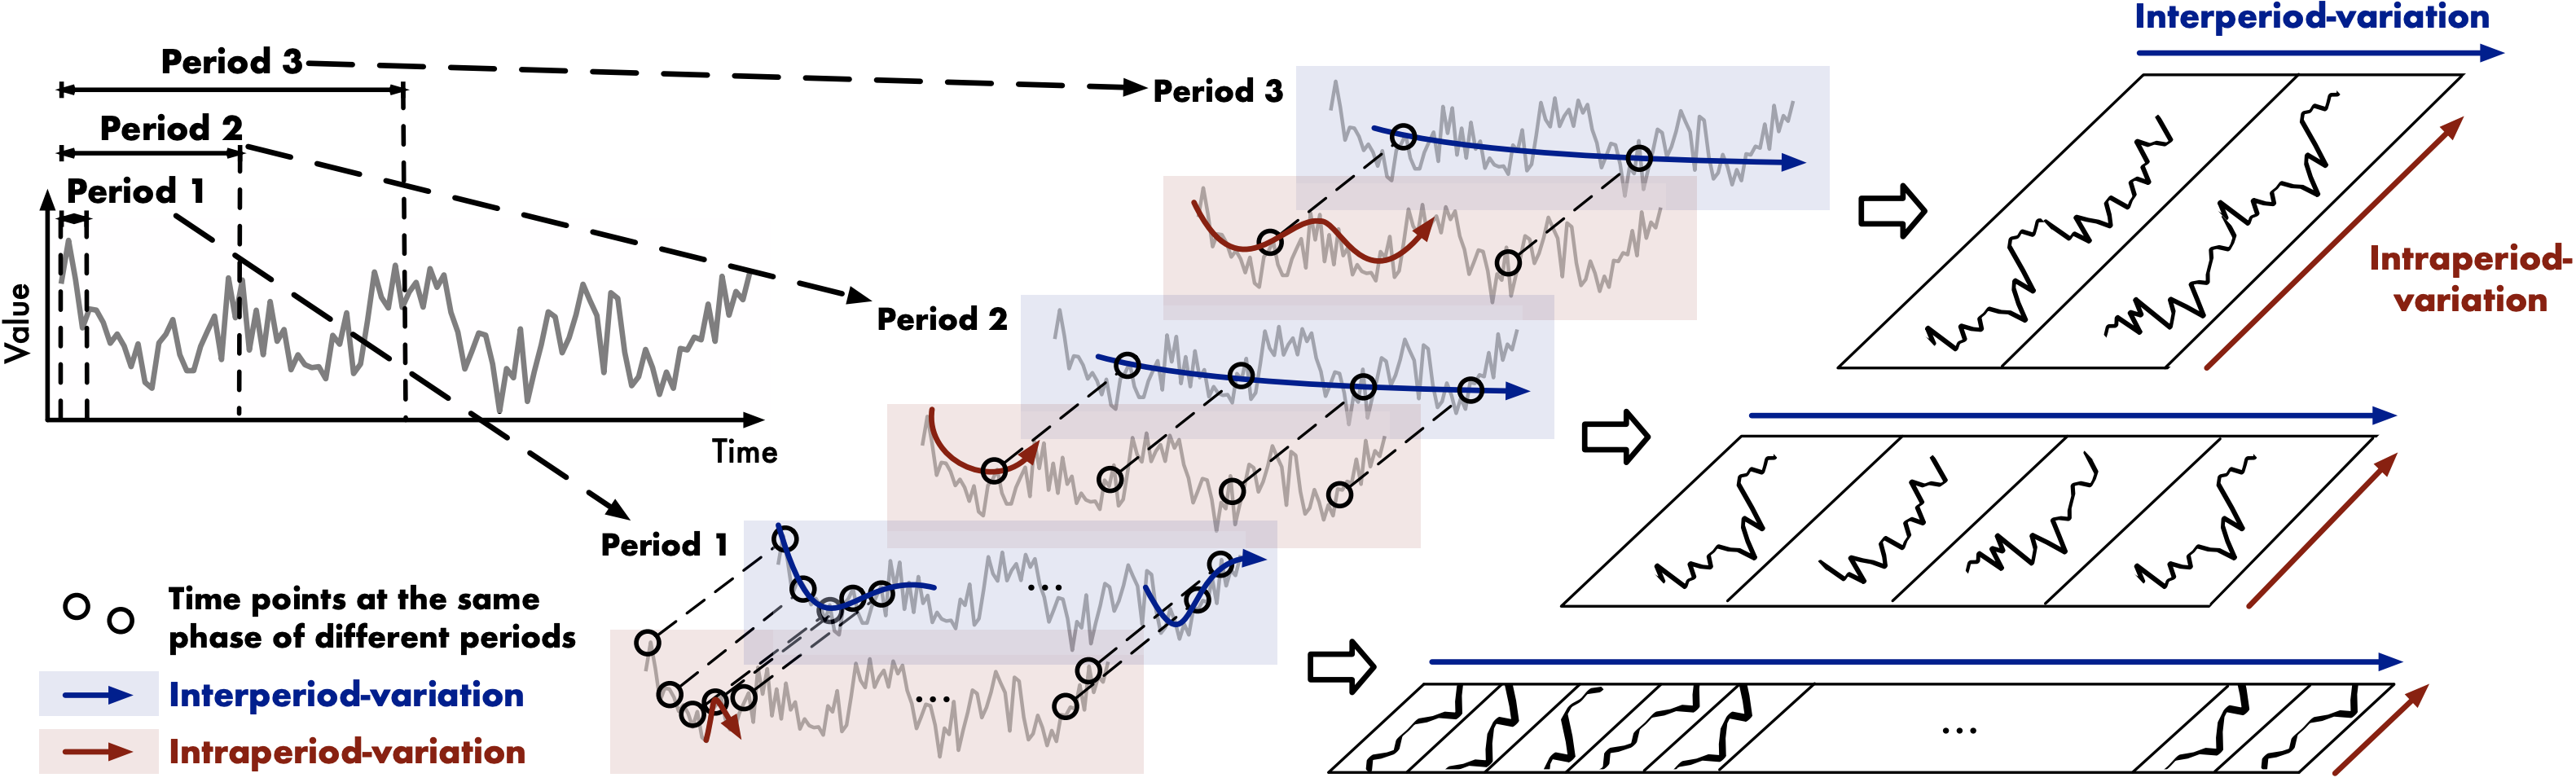
\includegraphics[width=0.4\textwidth]{img/2Dtensor.png}}
\caption{Chuyển đổi chuỗi thời gian 1D ban đầu thành một tập hợp các tensor 2D dựa trên nhiều chu kỳ.}
\label{fig}
\end{figure}